\section{Planning with Clearance Value Annotations}
\label{aha:annotations}
An annotation is simply a form of embedded domain knowledge that we store in our search graph and reference while computing a path plan. Such ideas are not new; some domain knowledge -- like terrain type --  is frequently pre-annotated into most grid maps. Terrain type annotations are useful because they allow us to determine which tiles are traversable by some class of agent and which are not and they are highly effective at pruning the search space for single-size agents. \\ \newline
Another type of annotation, recently emerging from the field of robotics, are clearance metrics. Frequently used to enrich probabilistic roadmaps, clearance values provide agents with information about the distance to the nearest obstacle at each navigable location \cite{geraerts04}. We will extend this idea and apply it to an octile grid map. We choose to work with grids because this representation is simple to build (especially compared to a roadmap) and very commonly applied in a wide range of shortest-path solvers. \\ \newline
On a grid map, a clearance value is associated with each octile and represents the dimensions of a theoretical square bounding volume that begins at the tile being evaluated and is expanded until it intersects an obstacle. The length or width of of the volume is taken as the clearance value at that location. This is an important measurement because it guarantees that the area subsumed by the bounding box is homogenous (topographically speaking).
To refine this idea, we will say that each traversable tile starts out with a minimum \emph{base clearance} of 1 while tiles marked as non-traversable (or those outside the grid map) always have a clearance value of 0. Once we have derived a clearance value, we use an additional few bytes of memory to annotate the corresponding node in our graph. Figure \ref{aha-fig:calculatingclearance} gives a quick overview of our technique. In \ref{aha-fig:calculatingclearance}(a) we present a simple map region and the target tile with base clearance. (b) and (c) show the first two successful expansions of the bounding volume; the third (d), fails. Finally, \ref{aha-fig:calculatingclearance}(d) shows the resultant clearance values for the entire region; we omit obstacle clearances which are all zero.

\begin{figure}[htbp]
        \caption{\emph{Determining maximal clearance} }
        \begin{center}
                        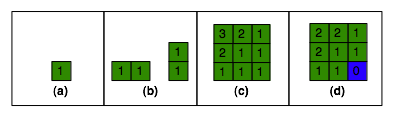
\includegraphics[scale=0.42]{diagrams/calculatingclearance.png}
        \end{center}
        \label{aha-fig:calculatingclearance}
\end{figure}

Although this approach is highly effective, it breaks down when there are multiple terrain types near some location. If we have large agents for example some may be able to traverse the tile and surrounding area while others not. For this reason, probabilistic roadmap methods using clearance are always limited to a single terrain type in the literature. To overcome this problem we propose embedding several clearance values at each fixed point in the environment, each one measuring the nearest-obstacle distance for every type of agent capability.  Capability in this case simply refers to a proper subset of the available terrain types found in our grid environment. Furthermore, we will henceforth refer to agents that can traverse several types of terrain as \emph{multi-capable}.

The process for calculating capability clearances is identical to that described until now with only one minor difference: we need to specify a target capability which we use to calculate the right clearance value. During processing, any tile we encounter that is not traversable for the given capability we will refer to as a \emph{soft obstacle} and assign it a clearance value of 0 for that capability. Tiles which are not traversable by any capability are said to be \emph{hard obstacles} and always assigned 0.  We continue in this manner for each available capability until all map tiles have been processed. Figure \ref{aha-fig:annotations} shows the results of different clearance value annotations we embedded into a tiny map during development. This map features two terrain types (represented by white and gray tiles respectively). On the left we show clearance values for all single-terrain capabilities. On the right, we compute clearance values for the capability combining the two terrain types. Again, we omit zero-values for obstacles.

Having outlined the basic approach, we can easily derive algorithm \ref{aha-alg:calculatingclearance} for computing all grid clearances. The precise implementation details of where to store clearances are not important. We opted to add attributes to our node data structures for simplicity; a better method would be to use compact tables.

\input algorithms/alg1_calculateclearance

Note that $t$ is a traversable tile in our grid map, and $t_{E}$, $t_{S}$ and $t_{SE}$ are octile neighbours (not necessarily traversable) in the stated directions.

\begin{figure}[htbp]
        \caption{\emph{Single terrain and multi-terrain clearance value annotations.} }
        \begin{center}
                        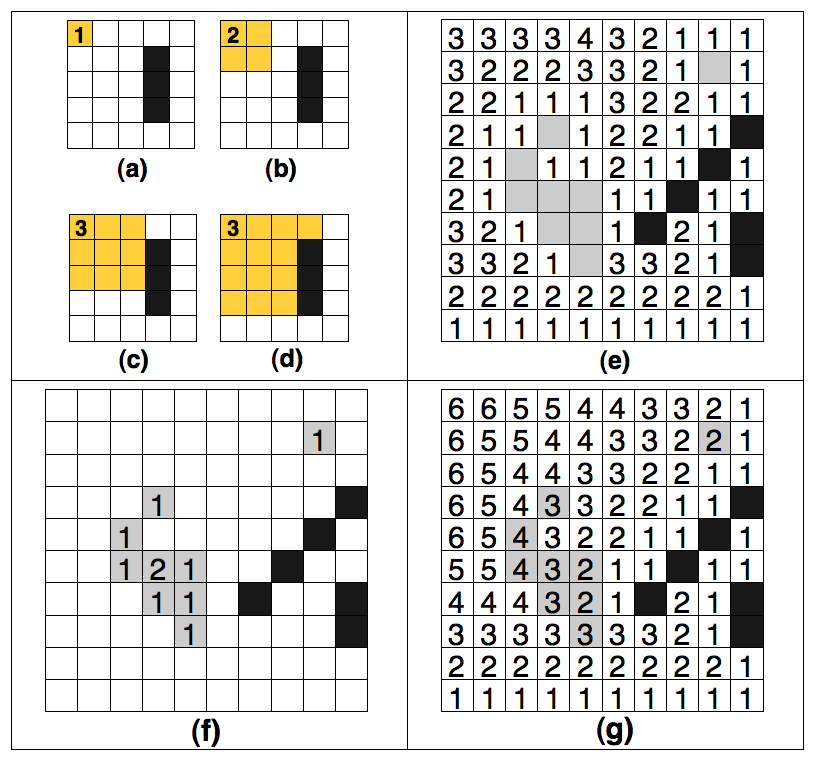
\includegraphics[scale=0.25]{diagrams/annotations.png}
        \end{center}
        \label{aha-fig:annotations}
\end{figure}

If we assume a capability exists for each combination of available terrain types, the exact number of annotations required for the initial grid map is given by:
\begin{equation}
N*2^t/2 - |N_{HO}|
\label{aha-eq:gridannotations}
\end{equation}

Where $t$ is the number of terrains on the map, $N$ is the set of all nodes in the map and $N_{HO}$ is the set of hard obstacles. \\ \newline
We derive this formula by noting that each node in the grid has a particular terrain type. It logically follows that each tile will only be traversable by a capability which includes the tile's terrain type meaning we do not need to unnecessarily store 0 clearance values. Similarly, we also avoid storing 0 values for hard obstacles.

